\subsection{Flight control board}

På figur \ref{fig:ibd_flightcontrolboard} vises ibd til Flight control. Flight control består af Flight control board og motor control. Flight control boardet kommunikerer med main controlleren via seriel kommunikation og 6 PWM signaler. Kompas information sendes vi den serielle kommunikation, og PWM signalerne bestemmer hvordan motorerne skal rotere. 

\begin{figure}[H]
\centering
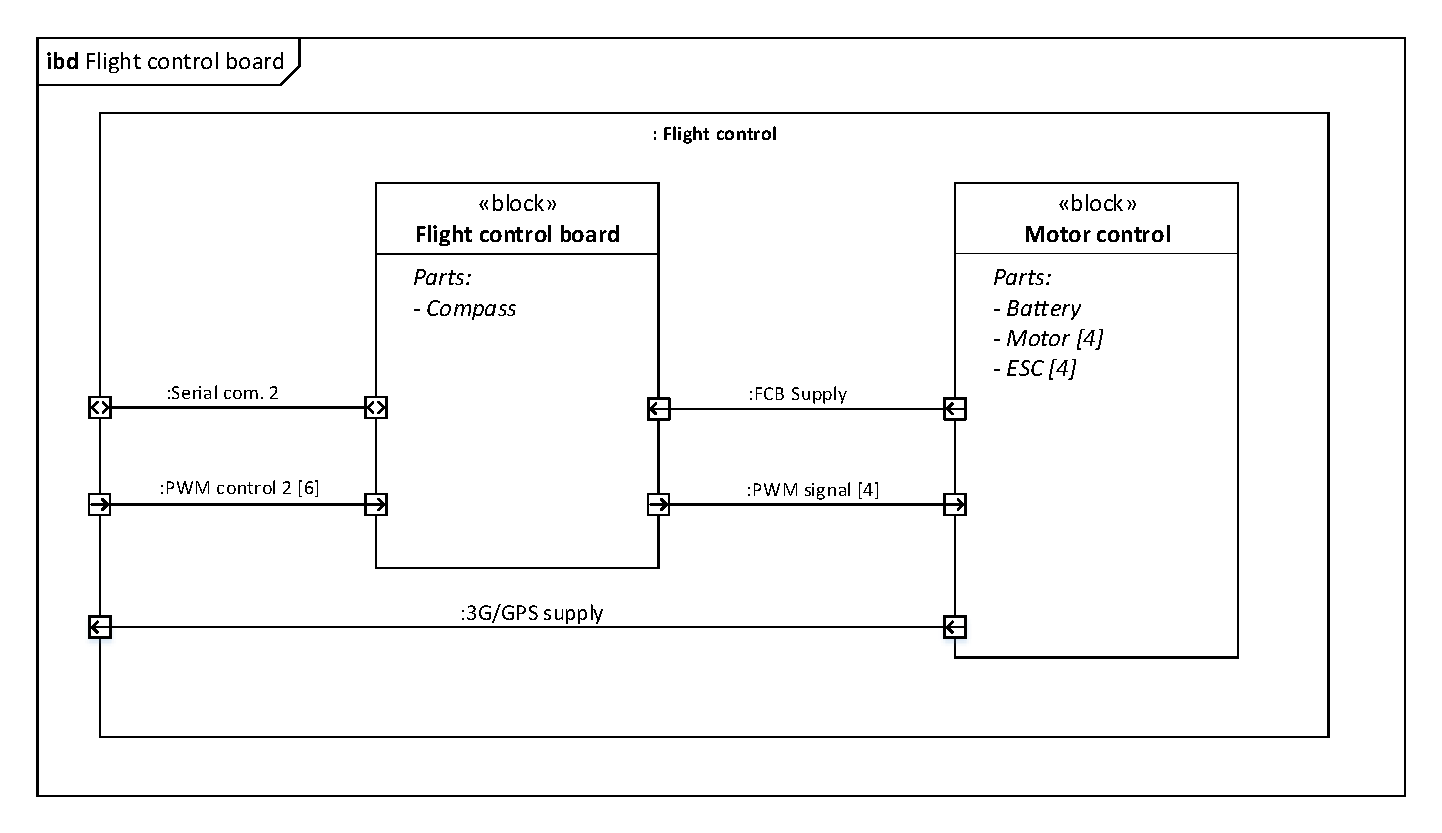
\includegraphics[width=1\textwidth]{Billeder/IBD/ibd5_flightcontrolboard.pdf}
\vspace{-1cm}
\caption{Ibd - flight control board}
\label{fig:ibd_flightcontrolboard}
\end{figure}

\begin{table}[H]
	\centering
		\begin{tabular}{|p{2.6 cm}|p{4.9 cm}|p{2.5 cm}|p{2.5 cm}|} 
		\hline
			\textbf{Signal navn} 	& \textbf{Signal beskrivelse}		& \textbf{Out} 				& \textbf{In}     \\ \hline
			Serial com. 2 & RX / TX. signal. & Arduino. & Flight control board.			    \\ \hline
			PWM control [6] & 50 Hz 6 kanals signal & Arduino. & Flight control board.				\\ \hline
			FCB supply &  Forsyning til flight contorl boarded. 5V DC & Motor control. & Flight control board.	\\ \hline
			PWM signal [4] & 400 Hz 4 kanals signal, Duty cycle mellem 40-80 $\%$. & Fligt control board. & Motor control.   \\ \hline 
			3G/GPS supply & 5V forsyning. & Motor control. & 3G/GPS.  \\ \hline 
		\end{tabular}
	\caption{Forbindelser til: Ibd - flight control board. }
	\label{tab:ibd_Flight_control_board}
\end{table}



